\chapter{Paths and circuits}

This chapter focuses on two types of paths in graphs:
\begin{itemize}
\item An \key{Eulerian path} is a path that
goes through each edge exactly once.
\item A \key{Hamiltonian path} is a path
that visits each node exactly once.
\end{itemize}
While Eulerian and Hamiltonian paths look like
similar concepts at first glance,
the computational problems related to them
are very different.
It turns out that there is a simple rule that
determines whether a graph contains an Eulerian path
and there is also an efficient algorithm to
find a such path if it exists.
On the contrary, checking the existence of a Hamiltonian path is a NP-hard
problem and no efficient algorithm is known for solving the problem.

\section{Eulerian paths}

\index{Eulerian path}

An \key{Eulerian path} is a path
that goes exactly once through each edge in the graph.
For example, the graph
\begin{center}
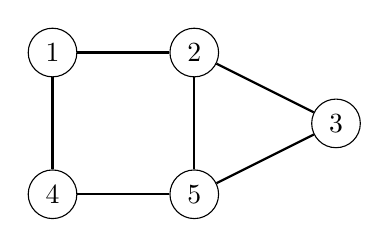
\begin{tikzpicture}[scale=0.9]
\node[draw, circle] (1) at (1,5) {$1$};
\node[draw, circle] (2) at (3,5) {$2$};
\node[draw, circle] (3) at (5,4) {$3$};
\node[draw, circle] (4) at (1,3) {$4$};
\node[draw, circle] (5) at (3,3) {$5$};

\path[draw,thick,-] (1) -- (2);
\path[draw,thick,-] (2) -- (3);
\path[draw,thick,-] (1) -- (4);
\path[draw,thick,-] (3) -- (5);
\path[draw,thick,-] (2) -- (5);
\path[draw,thick,-] (4) -- (5);
\end{tikzpicture}
\end{center}
has an Eulerian path from node 2 to node 5:
\begin{center}
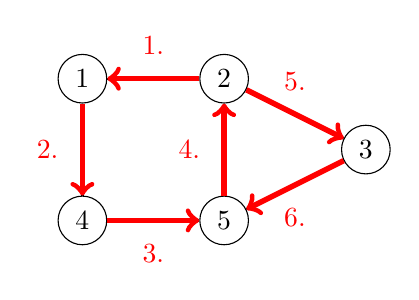
\begin{tikzpicture}[scale=0.9]
\node[draw, circle] (1) at (1,5) {$1$};
\node[draw, circle] (2) at (3,5) {$2$};
\node[draw, circle] (3) at (5,4) {$3$};
\node[draw, circle] (4) at (1,3) {$4$};
\node[draw, circle] (5) at (3,3) {$5$};

\path[draw,thick,-] (1) -- (2);
\path[draw,thick,-] (2) -- (3);
\path[draw,thick,-] (1) -- (4);
\path[draw,thick,-] (3) -- (5);
\path[draw,thick,-] (2) -- (5);
\path[draw,thick,-] (4) -- (5);

\path[draw=red,thick,->,line width=2pt] (2) -- node[font=\small,label={[red]north:1.}] {} (1);
\path[draw=red,thick,->,line width=2pt] (1) -- node[font=\small,label={[red]left:2.}] {} (4);
\path[draw=red,thick,->,line width=2pt] (4) -- node[font=\small,label={[red]south:3.}] {} (5);
\path[draw=red,thick,->,line width=2pt] (5) -- node[font=\small,label={[red]left:4.}] {} (2);
\path[draw=red,thick,->,line width=2pt] (2) -- node[font=\small,label={[red]north:5.}] {} (3);
\path[draw=red,thick,->,line width=2pt] (3) -- node[font=\small,label={[red]south:6.}] {} (5);
\end{tikzpicture}
\end{center}
\index{Eulerian circuit}
An \key{Eulerian circuit}
is an Eulerian path that starts and ends
at the same node.
For example, the graph
\begin{center}
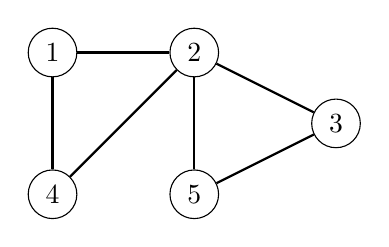
\begin{tikzpicture}[scale=0.9]
\node[draw, circle] (1) at (1,5) {$1$};
\node[draw, circle] (2) at (3,5) {$2$};
\node[draw, circle] (3) at (5,4) {$3$};
\node[draw, circle] (4) at (1,3) {$4$};
\node[draw, circle] (5) at (3,3) {$5$};

\path[draw,thick,-] (1) -- (2);
\path[draw,thick,-] (2) -- (3);
\path[draw,thick,-] (1) -- (4);
\path[draw,thick,-] (3) -- (5);
\path[draw,thick,-] (2) -- (5);
\path[draw,thick,-] (2) -- (4);
\end{tikzpicture}
\end{center}
has an Eulerian circuit that starts and ends at node 1:
\begin{center}
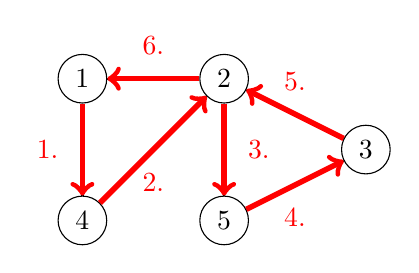
\begin{tikzpicture}[scale=0.9]
\node[draw, circle] (1) at (1,5) {$1$};
\node[draw, circle] (2) at (3,5) {$2$};
\node[draw, circle] (3) at (5,4) {$3$};
\node[draw, circle] (4) at (1,3) {$4$};
\node[draw, circle] (5) at (3,3) {$5$};

\path[draw,thick,-] (1) -- (2);
\path[draw,thick,-] (2) -- (3);
\path[draw,thick,-] (1) -- (4);
\path[draw,thick,-] (3) -- (5);
\path[draw,thick,-] (2) -- (5);
\path[draw,thick,-] (2) -- (4);

\path[draw=red,thick,->,line width=2pt] (1) -- node[font=\small,label={[red]left:1.}] {} (4);
\path[draw=red,thick,->,line width=2pt] (4) -- node[font=\small,label={[red]south:2.}] {} (2);
\path[draw=red,thick,->,line width=2pt] (2) -- node[font=\small,label={[red]right:3.}] {} (5);
\path[draw=red,thick,->,line width=2pt] (5) -- node[font=\small,label={[red]south:4.}] {} (3);
\path[draw=red,thick,->,line width=2pt] (3) -- node[font=\small,label={[red]north:5.}] {} (2);
\path[draw=red,thick,->,line width=2pt] (2) -- node[font=\small,label={[red]north:6.}] {} (1);
\end{tikzpicture}
\end{center}

\subsubsection{Existence}

The existence of Eulerian paths and circuits
depends on the degrees of the nodes in the graph.
First, an undirected graph has an Eulerian path if all the edges
belong to the same connected component and
\begin{itemize}
\item the degree of each node is even \emph{or}
\item the degree of exactly two nodes is odd,
and the degree of all other nodes is even.
\end{itemize}

In the first case, each Eulerian path in the graph
is also an Eulerian circuit.
In the second case, the odd-degree nodes are the starting
and ending nodes of an Eulerian path which is not an Eulerian circuit.

\begin{samepage}
For example, in the graph
\begin{center}
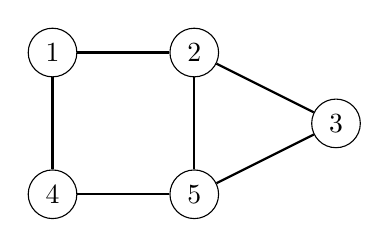
\begin{tikzpicture}[scale=0.9]
\node[draw, circle] (1) at (1,5) {$1$};
\node[draw, circle] (2) at (3,5) {$2$};
\node[draw, circle] (3) at (5,4) {$3$};
\node[draw, circle] (4) at (1,3) {$4$};
\node[draw, circle] (5) at (3,3) {$5$};

\path[draw,thick,-] (1) -- (2);
\path[draw,thick,-] (2) -- (3);
\path[draw,thick,-] (1) -- (4);
\path[draw,thick,-] (3) -- (5);
\path[draw,thick,-] (2) -- (5);
\path[draw,thick,-] (4) -- (5);
\end{tikzpicture}
\end{center}
\end{samepage}
nodes 1, 3 and 4 have a degree of 2,
and nodes 2 and 5 have a degree of 3.
Exactly two nodes have an even degree,
so there is an Eulerian path between nodes 2 and 5,
but the graph does not contain an Eulerian circuit.

In a directed graph,
we focus on indegrees and outdegrees
of the nodes of the graph.
A directed graph contains an Eulerian path
if all the edges belong to the same strongly
connected component and
\begin{itemize}
\item in each node, the indegree equals the outdegree, \emph{or}
\item in one node, the indegree is one larger than the outdegree,
in another node, the outdegree is one larger than the indegree,
and all other nodes, the indegree equals the outdegree.
\end{itemize}

In the first case, each Eulerian path in the graph
is also an Eulerian circuit,
and in the second case, the graph contains an Eulerian path
that begins at the node whose outdegree is larger
and ends at the node whose indegree is larger.

For example, in the graph
\begin{center}
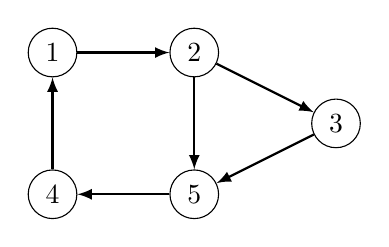
\begin{tikzpicture}[scale=0.9]
\node[draw, circle] (1) at (1,5) {$1$};
\node[draw, circle] (2) at (3,5) {$2$};
\node[draw, circle] (3) at (5,4) {$3$};
\node[draw, circle] (4) at (1,3) {$4$};
\node[draw, circle] (5) at (3,3) {$5$};

\path[draw,thick,->,>=latex] (1) -- (2);
\path[draw,thick,->,>=latex] (2) -- (3);
\path[draw,thick,->,>=latex] (4) -- (1);
\path[draw,thick,->,>=latex] (3) -- (5);
\path[draw,thick,->,>=latex] (2) -- (5);
\path[draw,thick,->,>=latex] (5) -- (4);
\end{tikzpicture}
\end{center}
nodes 1, 3 and 4 have both indegree 1 and outdegree 1,
node 2 has indegree 1 and outdegree 2,
and node 5 has indegree 2 and outdegree 1.
Hence, the graph contains an Eulerian path
from node 2 to node 5:
\begin{center}
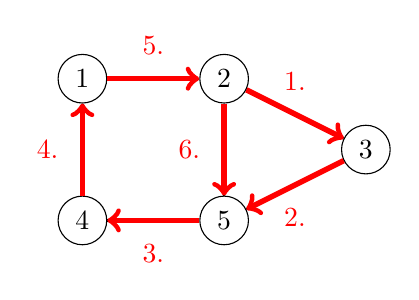
\begin{tikzpicture}[scale=0.9]
\node[draw, circle] (1) at (1,5) {$1$};
\node[draw, circle] (2) at (3,5) {$2$};
\node[draw, circle] (3) at (5,4) {$3$};
\node[draw, circle] (4) at (1,3) {$4$};
\node[draw, circle] (5) at (3,3) {$5$};

\path[draw,thick,-] (1) -- (2);
\path[draw,thick,-] (2) -- (3);
\path[draw,thick,-] (1) -- (4);
\path[draw,thick,-] (3) -- (5);
\path[draw,thick,-] (2) -- (5);
\path[draw,thick,-] (4) -- (5);

\path[draw=red,thick,->,line width=2pt] (2) -- node[font=\small,label={[red]north:1.}] {} (3);
\path[draw=red,thick,->,line width=2pt] (3) -- node[font=\small,label={[red]south:2.}] {} (5);
\path[draw=red,thick,->,line width=2pt] (5) -- node[font=\small,label={[red]south:3.}] {} (4);
\path[draw=red,thick,->,line width=2pt] (4) -- node[font=\small,label={[red]left:4.}] {} (1);
\path[draw=red,thick,->,line width=2pt] (1) -- node[font=\small,label={[red]north:5.}] {} (2);
\path[draw=red,thick,->,line width=2pt] (2) -- node[font=\small,label={[red]left:6.}] {} (5);
\end{tikzpicture}
\end{center}

\subsubsection{Hierholzer's algorithm}

\index{Hierholzer's algorithm}

\key{Hierholzer's algorithm} is an efficient
method for constructing
an Eulerian circuit.
The algorithm consists of several rounds,
each of which adds new edges to the circuit.
Of course, we assume that the graph contains
an Eulerian circuit; otherwise Hierholzer's
algorithm cannot find it.

First, the algorithm constructs a circuit that contains
some (not necessarily all) of the edges in the graph.
After this, the algorithm extends the circuit
step by step by adding subcircuits to it.
The process continues until all edges have been added
to the circuit.

The algorithm extends the circuit by always finding
a node $x$ that belongs to the circuit but has
an outgoing edge that is not included in the circuit.
The algorithm constructs a new path from node $x$
that only contains edges that are not yet in the circuit.
Sooner or later,
the path will return to the node $x$,
which creates a subcircuit.

If the graph only contains an Eulerian path,
we can still use Hierholzer's algorithm
to find it by adding an extra edge to the graph
and removing the edge after the circuit
has been constructed.
For example, in an undirected graph,
we add the extra edge between the two
odd-degree nodes.

Next we will see how Hierholzer's algorithm
constructs an Eulerian circuit in an undirected graph.

\subsubsection{Example}

\begin{samepage}
Let us consider the following graph:
\begin{center}
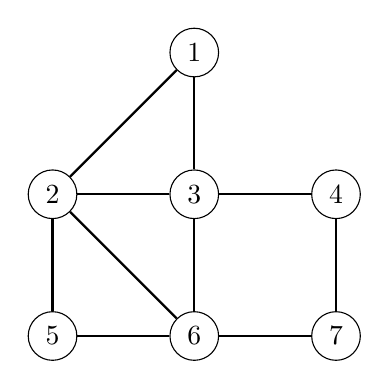
\begin{tikzpicture}[scale=0.9]
\node[draw, circle] (1) at (3,5) {$1$};
\node[draw, circle] (2) at (1,3) {$2$};
\node[draw, circle] (3) at (3,3) {$3$};
\node[draw, circle] (4) at (5,3) {$4$};
\node[draw, circle] (5) at (1,1) {$5$};
\node[draw, circle] (6) at (3,1) {$6$};
\node[draw, circle] (7) at (5,1) {$7$};

\path[draw,thick,-] (1) -- (2);
\path[draw,thick,-] (1) -- (3);
\path[draw,thick,-] (2) -- (3);
\path[draw,thick,-] (2) -- (5);
\path[draw,thick,-] (2) -- (6);
\path[draw,thick,-] (3) -- (4);
\path[draw,thick,-] (3) -- (6);
\path[draw,thick,-] (4) -- (7);
\path[draw,thick,-] (5) -- (6);
\path[draw,thick,-] (6) -- (7);
\end{tikzpicture}
\end{center}
\end{samepage}

\begin{samepage}
Suppose that the algorithm first creates a circuit
that begins at node 1.
A possible circuit is
$1 \rightarrow 2 \rightarrow 3 \rightarrow 1$:
\begin{center}
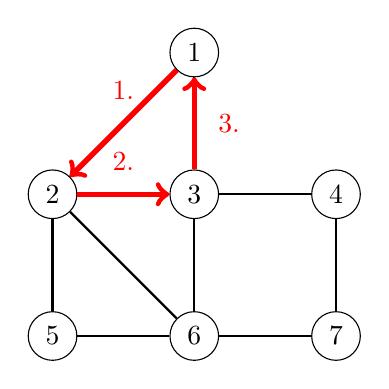
\begin{tikzpicture}[scale=0.9]
\node[draw, circle] (1) at (3,5) {$1$};
\node[draw, circle] (2) at (1,3) {$2$};
\node[draw, circle] (3) at (3,3) {$3$};
\node[draw, circle] (4) at (5,3) {$4$};
\node[draw, circle] (5) at (1,1) {$5$};
\node[draw, circle] (6) at (3,1) {$6$};
\node[draw, circle] (7) at (5,1) {$7$};

\path[draw,thick,-] (1) -- (2);
\path[draw,thick,-] (1) -- (3);
\path[draw,thick,-] (2) -- (3);
\path[draw,thick,-] (2) -- (5);
\path[draw,thick,-] (2) -- (6);
\path[draw,thick,-] (3) -- (4);
\path[draw,thick,-] (3) -- (6);
\path[draw,thick,-] (4) -- (7);
\path[draw,thick,-] (5) -- (6);
\path[draw,thick,-] (6) -- (7);

\path[draw=red,thick,->,line width=2pt] (1) -- node[font=\small,label={[red]north:1.}] {} (2);
\path[draw=red,thick,->,line width=2pt] (2) -- node[font=\small,label={[red]north:2.}] {} (3);
\path[draw=red,thick,->,line width=2pt] (3) -- node[font=\small,label={[red]east:3.}] {} (1);
\end{tikzpicture}
\end{center}
\end{samepage}
After this, the algorithm adds
the subcircuit
$2 \rightarrow 5 \rightarrow 6 \rightarrow 2$
to the circuit:
\begin{center}
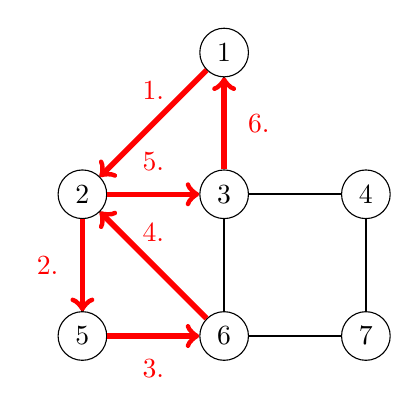
\begin{tikzpicture}[scale=0.9]
\node[draw, circle] (1) at (3,5) {$1$};
\node[draw, circle] (2) at (1,3) {$2$};
\node[draw, circle] (3) at (3,3) {$3$};
\node[draw, circle] (4) at (5,3) {$4$};
\node[draw, circle] (5) at (1,1) {$5$};
\node[draw, circle] (6) at (3,1) {$6$};
\node[draw, circle] (7) at (5,1) {$7$};

\path[draw,thick,-] (1) -- (2);
\path[draw,thick,-] (1) -- (3);
\path[draw,thick,-] (2) -- (3);
\path[draw,thick,-] (2) -- (5);
\path[draw,thick,-] (2) -- (6);
\path[draw,thick,-] (3) -- (4);
\path[draw,thick,-] (3) -- (6);
\path[draw,thick,-] (4) -- (7);
\path[draw,thick,-] (5) -- (6);
\path[draw,thick,-] (6) -- (7);

\path[draw=red,thick,->,line width=2pt] (1) -- node[font=\small,label={[red]north:1.}] {} (2);
\path[draw=red,thick,->,line width=2pt] (2) -- node[font=\small,label={[red]west:2.}] {} (5);
\path[draw=red,thick,->,line width=2pt] (5) -- node[font=\small,label={[red]south:3.}] {} (6);
\path[draw=red,thick,->,line width=2pt] (6) -- node[font=\small,label={[red]north:4.}] {} (2);
\path[draw=red,thick,->,line width=2pt] (2) -- node[font=\small,label={[red]north:5.}] {} (3);
\path[draw=red,thick,->,line width=2pt] (3) -- node[font=\small,label={[red]east:6.}] {} (1);
\end{tikzpicture}
\end{center}
Finally, the algorithm adds the subcircuit
$6 \rightarrow 3 \rightarrow 4 \rightarrow 7 \rightarrow 6$
to the circuit:
\begin{center}
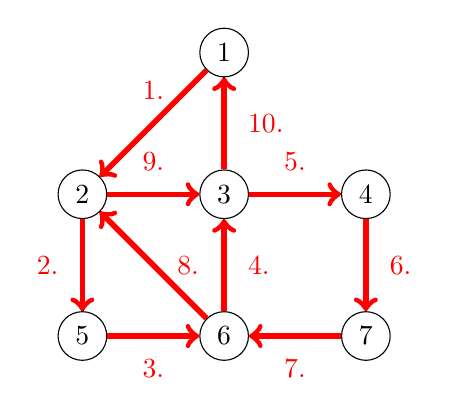
\begin{tikzpicture}[scale=0.9]
\node[draw, circle] (1) at (3,5) {$1$};
\node[draw, circle] (2) at (1,3) {$2$};
\node[draw, circle] (3) at (3,3) {$3$};
\node[draw, circle] (4) at (5,3) {$4$};
\node[draw, circle] (5) at (1,1) {$5$};
\node[draw, circle] (6) at (3,1) {$6$};
\node[draw, circle] (7) at (5,1) {$7$};

\path[draw,thick,-] (1) -- (2);
\path[draw,thick,-] (1) -- (3);
\path[draw,thick,-] (2) -- (3);
\path[draw,thick,-] (2) -- (5);
\path[draw,thick,-] (2) -- (6);
\path[draw,thick,-] (3) -- (4);
\path[draw,thick,-] (3) -- (6);
\path[draw,thick,-] (4) -- (7);
\path[draw,thick,-] (5) -- (6);
\path[draw,thick,-] (6) -- (7);

\path[draw=red,thick,->,line width=2pt] (1) -- node[font=\small,label={[red]north:1.}] {} (2);
\path[draw=red,thick,->,line width=2pt] (2) -- node[font=\small,label={[red]west:2.}] {} (5);
\path[draw=red,thick,->,line width=2pt] (5) -- node[font=\small,label={[red]south:3.}] {} (6);
\path[draw=red,thick,->,line width=2pt] (6) -- node[font=\small,label={[red]east:4.}] {} (3);
\path[draw=red,thick,->,line width=2pt] (3) -- node[font=\small,label={[red]north:5.}] {} (4);
\path[draw=red,thick,->,line width=2pt] (4) -- node[font=\small,label={[red]east:6.}] {} (7);
\path[draw=red,thick,->,line width=2pt] (7) -- node[font=\small,label={[red]south:7.}] {} (6);
\path[draw=red,thick,->,line width=2pt] (6) -- node[font=\small,label={[red]right:8.}] {} (2);
\path[draw=red,thick,->,line width=2pt] (2) -- node[font=\small,label={[red]north:9.}] {} (3);
\path[draw=red,thick,->,line width=2pt] (3) -- node[font=\small,label={[red]east:10.}] {} (1);
\end{tikzpicture}
\end{center}
Now all edges are included in the circuit,
so we have successfully constructed an Eulerian circuit.

\section{Hamiltonian paths}

\index{Hamiltonian path}

A \key{Hamiltonian path} is a path
that visits each node in the graph exactly once.
For example, the graph
\begin{center}
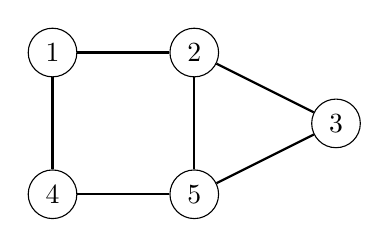
\begin{tikzpicture}[scale=0.9]
\node[draw, circle] (1) at (1,5) {$1$};
\node[draw, circle] (2) at (3,5) {$2$};
\node[draw, circle] (3) at (5,4) {$3$};
\node[draw, circle] (4) at (1,3) {$4$};
\node[draw, circle] (5) at (3,3) {$5$};

\path[draw,thick,-] (1) -- (2);
\path[draw,thick,-] (2) -- (3);
\path[draw,thick,-] (1) -- (4);
\path[draw,thick,-] (3) -- (5);
\path[draw,thick,-] (2) -- (5);
\path[draw,thick,-] (4) -- (5);
\end{tikzpicture}
\end{center}
contains a Hamiltonian path from node 1 to node 3:
\begin{center}
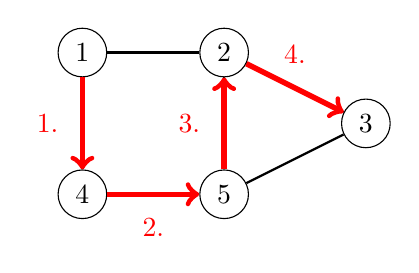
\begin{tikzpicture}[scale=0.9]
\node[draw, circle] (1) at (1,5) {$1$};
\node[draw, circle] (2) at (3,5) {$2$};
\node[draw, circle] (3) at (5,4) {$3$};
\node[draw, circle] (4) at (1,3) {$4$};
\node[draw, circle] (5) at (3,3) {$5$};

\path[draw,thick,-] (1) -- (2);
\path[draw,thick,-] (2) -- (3);
\path[draw,thick,-] (1) -- (4);
\path[draw,thick,-] (3) -- (5);
\path[draw,thick,-] (2) -- (5);
\path[draw,thick,-] (4) -- (5);

\path[draw=red,thick,->,line width=2pt] (1) -- node[font=\small,label={[red]left:1.}] {} (4);
\path[draw=red,thick,->,line width=2pt] (4) -- node[font=\small,label={[red]south:2.}] {} (5);
\path[draw=red,thick,->,line width=2pt] (5) -- node[font=\small,label={[red]left:3.}] {} (2);
\path[draw=red,thick,->,line width=2pt] (2) -- node[font=\small,label={[red]north:4.}] {} (3);
\end{tikzpicture}
\end{center}

\index{Hamiltonian circuit}

If a Hamiltonian path begins and ends at the same node,
it is called a \key{Hamiltonian circuit}.
The graph above also has an Hamiltonian circuit
that begins and ends at node 1:
\begin{center}
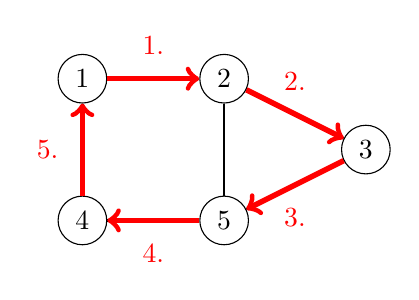
\begin{tikzpicture}[scale=0.9]
\node[draw, circle] (1) at (1,5) {$1$};
\node[draw, circle] (2) at (3,5) {$2$};
\node[draw, circle] (3) at (5,4) {$3$};
\node[draw, circle] (4) at (1,3) {$4$};
\node[draw, circle] (5) at (3,3) {$5$};

\path[draw,thick,-] (1) -- (2);
\path[draw,thick,-] (2) -- (3);
\path[draw,thick,-] (1) -- (4);
\path[draw,thick,-] (3) -- (5);
\path[draw,thick,-] (2) -- (5);
\path[draw,thick,-] (4) -- (5);

\path[draw=red,thick,->,line width=2pt] (1) -- node[font=\small,label={[red]north:1.}] {} (2);
\path[draw=red,thick,->,line width=2pt] (2) -- node[font=\small,label={[red]north:2.}] {} (3);
\path[draw=red,thick,->,line width=2pt] (3) -- node[font=\small,label={[red]south:3.}] {} (5);
\path[draw=red,thick,->,line width=2pt] (5) -- node[font=\small,label={[red]south:4.}] {} (4);
\path[draw=red,thick,->,line width=2pt] (4) -- node[font=\small,label={[red]left:5.}] {} (1);
\end{tikzpicture}
\end{center}

\subsubsection{Existence}

No efficient method is known for testing if a graph
contains a Hamiltonian path, but the problem is NP-hard.
Still, in some special cases we can be certain
that the graph contains a Hamiltonian path.

A simple observation is that if the graph is complete,
i.e., there is an edge between all pairs of nodes,
it also contains a Hamiltonian path.
Also stronger results have been achieved:

\begin{itemize}
\item
\index{Dirac's theorem}
\key{Dirac's theorem}:
If the degree of each node is at least $n/2$,
the graph contains a Hamiltonian path.
\item
\index{Ore's theorem}
\key{Ore's theorem}:
If the sum of degrees of each non-adjacent pair of nodes
is at least $n$,
the graph contains a Hamiltonian path.
\end{itemize}

A common property in these theorems and other results is
that they guarantee the existence of a Hamiltonian
if the graph has \emph{a large number} of edges.
This makes sense, because the more edges the graph contains,
the more possibilities there is to construct a Hamiltonian graph.

\subsubsection{Construction}

Since there is no efficient way to check if a Hamiltonian
path exists, it is clear that there is also no method
for constructing the path efficiently, because otherwise
we could just try to construct the path and see
whether it exists.

A simple way to search for a Hamiltonian path is
to use a backtracking algorithm that goes through all
possible ways to construct the path.
The time complexity of such an algorithm is at least $O(n!)$,
because there are $n!$ different ways to choose the order of $n$ nodes.

A more efficient solution is based on dynamic programming
(see Chapter 10.4).
The idea is to define a function $f(s,x)$,
where $s$ is a subset of nodes and $x$
is one of the nodes in the subset.
The function indicates whether there is a Hamiltonian path
that visits the nodes in $s$ and ends at node $x$.
It is possible to implement this solution in $O(2^n n^2)$ time.

\section{De Bruijn sequences}

\index{De Bruijn sequence}

A \key{De Bruijn sequence} is a string that contains
every string of length $n$
exactly once as a substring, for a fixed
alphabet of $k$ characters.
The length of such a string is 
$k^n+n-1$ characters.
For example, when $n=3$ and $k=2$,
an example of a De Bruijn sequence is
\[0001011100.\]
The substrings of this string are all
combinations of three bits:
000, 001, 010, 011, 100, 101, 110 and 111.

It turns out that each De Bruijn sequence
corresponds to an Eulerian circuit in a graph.
The idea is to construct the graph so that
each node contains a combination of $n-1$ characters
and each edge adds one character to the string.
The following graph corresponds to the above example:

\begin{center}
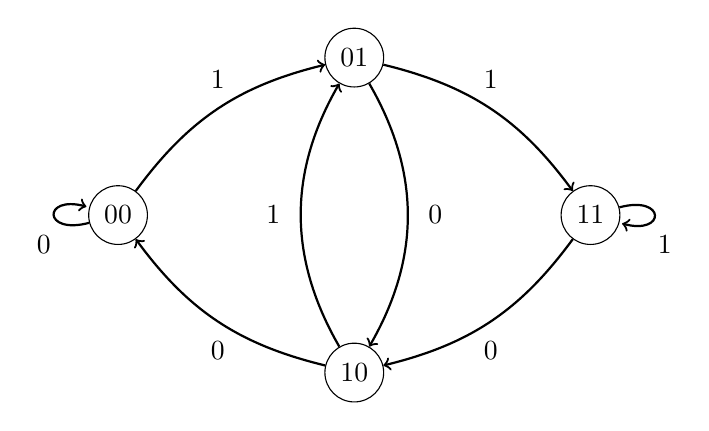
\begin{tikzpicture}
\node[draw, circle] (00) at (-3,0) {00};
\node[draw, circle] (11) at (3,0) {11};
\node[draw, circle] (01) at (0,2) {01};
\node[draw, circle] (10) at (0,-2) {10};

\path[draw,thick,->] (00) edge [bend left=20] node[font=\small,label=1] {} (01);
\path[draw,thick,->] (01) edge [bend left=20] node[font=\small,label=1] {} (11);
\path[draw,thick,->] (11) edge [bend left=20] node[font=\small,label=below:0] {} (10);
\path[draw,thick,->] (10) edge [bend left=20] node[font=\small,label=below:0] {} (00);

\path[draw,thick,->] (01) edge [bend left=30] node[font=\small,label=right:0] {} (10);
\path[draw,thick,->] (10) edge [bend left=30] node[font=\small,label=left:1] {} (01);

\path[draw,thick,-] (00) edge [loop left] node[font=\small,label=below:0] {} (00);
\path[draw,thick,-] (11) edge [loop right] node[font=\small,label=below:1] {} (11);
\end{tikzpicture}
\end{center}

An Eulerian path in this graph corresponds to a string
that contains all strings of length $n$.
The string contains the characters of the starting node
and all characters in the edges.
The starting node has $n-1$ characters
and there are $k^n$ characters in the edges,
so the length of the string is $k^n+n-1$.

\section{Knight's tours}

\index{knight's tour}

A \key{knight's tour} is a sequence of moves
of a knight on an $n \times n$ chessboard
following the rules of chess such that the knight
visits each square exactly once.
The tour is \key{closed} if the knight finally
returns to the starting square and
otherwise the tour is \key{open}.

For example, here is an open knight's tour on a $5 \times 5$ board:

\begin{center}
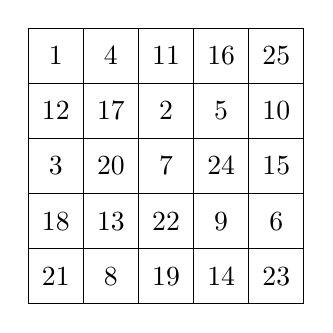
\begin{tikzpicture}[scale=0.7]
\draw (0,0) grid (5,5);
\node at (0.5,4.5) {$1$};
\node at (1.5,4.5) {$4$};
\node at (2.5,4.5) {$11$};
\node at (3.5,4.5) {$16$};
\node at (4.5,4.5) {$25$};
\node at (0.5,3.5) {$12$};
\node at (1.5,3.5) {$17$};
\node at (2.5,3.5) {$2$};
\node at (3.5,3.5) {$5$};
\node at (4.5,3.5) {$10$};
\node at (0.5,2.5) {$3$};
\node at (1.5,2.5) {$20$};
\node at (2.5,2.5) {$7$};
\node at (3.5,2.5) {$24$};
\node at (4.5,2.5) {$15$};
\node at (0.5,1.5) {$18$};
\node at (1.5,1.5) {$13$};
\node at (2.5,1.5) {$22$};
\node at (3.5,1.5) {$9$};
\node at (4.5,1.5) {$6$};
\node at (0.5,0.5) {$21$};
\node at (1.5,0.5) {$8$};
\node at (2.5,0.5) {$19$};
\node at (3.5,0.5) {$14$};
\node at (4.5,0.5) {$23$};
\end{tikzpicture}
\end{center}

A knight's tour corresponds to a Hamiltonian path in a graph
whose nodes represent the squares of the board
and two nodes are connected with an edge if a knight
can move between the squares according to the rules of chess.

A natural way to construct a knight's tour is to use backtracking.
The search can be made more efficient by using
\key{heuristics} that attempt to guide the knight so that
a complete tour will be found quickly.

\subsubsection{Warnsdorff's rule}

\index{heuristic}
\index{Warnsdorff's rule}

\key{Warnsdorff's rule} is a simple and effective heuristic
for finding a knight's tour.
Using the rule, it is possible to efficiently construct a tour
even on a large board.
The idea is to always move the knight so that it ends up
in a square where the number of possible moves is as
\emph{small} as possible.

For example, in the following situation there are five
possible squares to which the knight can move:
\begin{center}
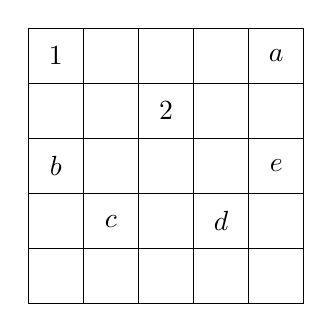
\begin{tikzpicture}[scale=0.7]
\draw (0,0) grid (5,5);
\node at (0.5,4.5) {$1$};
\node at (2.5,3.5) {$2$};
\node at (4.5,4.5) {$a$};
\node at (0.5,2.5) {$b$};
\node at (4.5,2.5) {$e$};
\node at (1.5,1.5) {$c$};
\node at (3.5,1.5) {$d$};
\end{tikzpicture}
\end{center}
In this situation, Warnsdorff's rule moves the knight to square $a$,
because after this choice, there is only a single possible move.
The other choices would move the knight to squares where
there would be three moves available.


